
\documentclass[
brazilian,
12pt,
a4paper,
oneside,
chapter=TITLE,
section=TITLE
]{setup/abnt_ufsc_tex}

\titulo{
    Relatório de Execução do Projeto \\
    \large INE5617-07238 - Gerência de Projetos
}
\local{Florianópolis -- SC}
\ano{2025}
\autor{
    Manuela Schmitz \and Gabriel Avila \and Gustavo Cortez de Brito \and Thayssa Yasmin Alcantara de Godoi \\
    Universidade Federal de Santa Catarina (UFSC) \\
    Curso de Sistemas de Informação
}
\instituicao{Universidade Federal de Santa Catarina (UFSC)}
\instituicaosigla{UFSC}
\programa{Curso de Sistemas de Informação}
\tipotrabalho{Relatório de Execução do Projeto}
\data{10 de junho de 2025 \\ Florianópolis -- SC}

\hypersetup{
    pdfsubject={Relatório de Execução do Projeto},
    pdfcreator={LaTeX},
    pdftitle={Relatório de Execução do Projeto - INE5617-07238},
    pdfauthor={Manuela Schmitz, Gabriel Avila, Gustavo Cortez de Brito, Thayssa Yasmin Alcantara de Godoi},
    pdfkeywords={Gerência de Projetos, UFSC, Relatório de Execução, INE5617},
}
%----------------------------------------------------------------------------------------
%   Thesis Tweaks and Utilities
%----------------------------------------------------------------------------------------
\makeatletter


% Uncomment this if you are debugging pages' badness Underfull & Overflow
% https://tex.stackexchange.com/questions/115908/geometry-showframe-landscape
% https://tex.stackexchange.com/questions/387077/what-is-the-difference-between-usepackageshowframe-and-usepackageshowframe
% https://tex.stackexchange.com/questions/387257/how-to-do-the-memoir-headings-fix-but-not-have-my-text-going-over-the-page-botto
% https://tex.stackexchange.com/questions/14508/print-page-margins-of-a-document
% \usepackage[showframe,pass]{geometry}

% To use the font Times New Roman, instead of the default LaTeX font
% more up-to-date than '\usepackage{mathptmx}'
% \usepackage{newtxtext}
% \usepackage{newtxmath}

% https://tex.stackexchange.com/questions/182569/how-to-manually-set-where-a-word-is-split
\hyphenation{Ge-la-im}
\hyphenation{Cis-la-ghi}

% Add missing translations for Portuguese
% https://tex.stackexchange.com/questions/8564/what-is-the-right-way-to-redefine-macros-defined-by-babel
\@ifpackageloaded{babel}{\@ifpackagewith{babel}{brazil}{\addto\captionsbrazil{%
  \renewcommand{\mytextpreliminarylistname}{Breve Sumário}
}}{}}{}
\@ifundefined{advisor}{\newcommand{\advisor}[2]{#1}}{}

% Selects a sans serif font family
% \renewcommand{\sfdefault}{cmss}

% Selects a monospaced (“typewriter”) font family
% \renewcommand{\ttdefault}{cmtt}

% Spacing between lines and paragraphs
% https://tex.stackexchange.com/questions/70212/ifpackageloaded-question
\@ifclassloaded{memoir}
{
  % New custom chapter style VZ14, see other chapters styles in:
  % http://repositorios.cpai.unb.br/ctan/info/latex-samples/MemoirChapStyles/MemoirChapStyles.pdf
  \newcommand\thickhrulefill{\leavevmode \leaders \hrule height 1ex \hfill \kern \z@}
  \makechapterstyle{VZ14} { %
    % \thispagestyle{empty}
    \setlength\beforechapskip{50pt}
    \setlength\midchapskip{20pt}
    \setlength\afterchapskip{20pt}
    \renewcommand\chapternamenum{}
    \renewcommand\printchaptername{}
    \renewcommand\chapnamefont{\Huge\scshape}
    \renewcommand\printchapternum {%
      \chapnamefont\null\thickhrulefill\quad
      \@chapapp\space\thechapter\quad\thickhrulefill
    }
    \renewcommand\printchapternonum {%
      \par\thickhrulefill\par\vskip\midchapskip
      \hrule\vskip\midchapskip
    }
    \renewcommand\chaptitlefont{\huge\scshape\centering}
    \renewcommand\afterchapternum {%
      \par\nobreak\vskip\midchapskip\hrule\vskip\midchapskip
    }
    \renewcommand\afterchaptertitle {%
      \par\vskip\midchapskip\hrule\nobreak\vskip\afterchapskip
    }
  }

  % Apply the style `VZ14` just created
  % \chapterstyle{VZ14}

  % http://mirrors.ibiblio.org/CTAN/macros/latex/contrib/memoir/memman.pdf
  \setlength\beforechapskip{0pt}
  \setlength\midchapskip{15pt}
  \setlength\afterchapskip{15pt}

  % Memoir: Warnings “The material used in the headers is too large” w/ accented titles
  % https://tex.stackexchange.com/questions/387293/how-to-change-the-page-layout-with-memoir
  \setheadfoot{30.0pt}{\footskip}
  \checkandfixthelayout
}{}

% Controlling the spacing between one paragraph and another
% Default value for UFSC 0.0cm
\setlength{\parskip}{\advisor{0.0cm}{0.2cm}}

% Paragraph size is given by
% Default value for UFSC 1.5cm
% \setlength{\parindent}{1.3cm}

% https://tex.stackexchange.com/questions/148647/how-to-remove-space-before-enumerate
% https://tex.stackexchange.com/questions/433543/behaviour-of-enumitem-setlist
\advisor{}{
    \setlist*[enumerate]{label=\arabic*,}
    \setlist*[enumerateoptional]{label=\arabic*,}

    % https://tex.stackexchange.com/questions/24454/space-after-float-with-h
    % https://tex.stackexchange.com/questions/23313/how-can-i-reduce-padding-after-figure
    \AtBeginEnvironment{figure}{
      \setlength{\intextsep}{5pt} % Vertical space above & below [h] floats
      % \setlength{\textfloatsep}{10pt} % Vertical space below (above) [t] ([b]) floats
      % \setlength{\abovecaptionskip}{10pt}
      % \setlength{\belowcaptionskip}{5pt}
    }

    % Patch the `abntex2` citacao environment removing the extra space from its top
    % https://tex.stackexchange.com/questions/300340/topsep-itemsep-partopsep-and-parsep-what-does-each-of-them-mean-and-wha
    \xpatchcmd{\citacao}
    {\list{}}
    {\list{}{\topsep=0pt}}
    {}
    {\FAILEDPATCHINGCITACAO}
}


% Color settings across the document
\@ifpackageloaded{xcolor}
{
  % RGB colors in absolute values from 0 to 255 by using `RGB` tag
  \definecolor{darkblue}{RGB}{26,13,178}

  % Colors names definitions as RGB colors in percentage notation by using `rgb` tag
  \definecolor{mygreen}{rgb}{0,0.6,0}
  \definecolor{mygray}{rgb}{0.5,0.5,0.5}
  \definecolor{mymauve}{rgb}{0.58,0,0.82}
  \definecolor{figcolor}{rgb}{1,0.4,0}
  \definecolor{tabcolor}{rgb}{1,0.4,0}
  \definecolor{eqncolor}{rgb}{1,0.4,0}
  \definecolor{linkcolor}{rgb}{1,0.4,0}
  \definecolor{citecolor}{rgb}{1,0.4,0}
  \definecolor{seccolor}{rgb}{0,0,1}
  \definecolor{abscolor}{rgb}{0,0,1}
  \definecolor{titlecolor}{rgb}{0,0,1}
  \definecolor{biocolor}{rgb}{0,0,1}
  \definecolor{blue}{RGB}{41,5,195}

  % PDF Hyperlinks settings
  \@ifpackageloaded{hyperref}
  {
    \hypersetup
    {
      colorlinks=true,     % false: boxed links; true: colored links
      linkcolor=darkblue,  % color of internal links
      citecolor=darkblue, % color of links to bibliography
      filecolor=black,     % color of file links
      urlcolor=\advisor{black}{darkgreen},
      bookmarksdepth=4,
      pdfencoding=auto,%
      psdextra,
    }
  }
}{}


% Filtering and Mapping Bibliographies
% \DeclareFieldFormat{url}{Disponível~em:\addspace\url{#1}}

% https://tex.stackexchange.com/questions/517526/how-to-make-biblatex-url-links-generated-with-brackets-around-it-url-correctly
\DeclareFieldFormat{url}{\bibstring{urlfrom}\addcolon\space\textless\url{#1}\textgreater}
\DefineBibliographyStrings{brazil}{urlfrom = {Disponível em}}
\DefineBibliographyStrings{english}{urlfrom = {Available from}}

% https://tex.stackexchange.com/questions/391695/is-possible-to-remove-the-link-color-of-the-comma-on-the-citation-link
% \DeclareFieldFormat{citehyperref}{#1}

% % https://tex.stackexchange.com/questions/203764/reduce-font-size-of-bibliography-overfull-bibliography
% \newcommand{\bibliographyfontsize}{\fontsize{10.0pt}{10.5pt}\selectfont}
% \renewcommand*{\bibfont}{\bibliographyfontsize}

% Uncomment this to insert the abstract into your bibliography entries when the abstract is available
% https://tex.stackexchange.com/questions/398666/how-to-correctly-insert-and-justify-abstract
\ifadvisor
\else
  \DeclareFieldFormat{abstract}%
  {%
    \par\justifying
    \begin{adjustwidth}{1cm}{}
      \textbf{\bibsentence\bibstring{abstract}:} #1
    \end{adjustwidth}
  }
  \renewbibmacro*{finentry}%
  {%
    \iffieldundef{abstract}
    {\finentry}
    {\finentrypunct
      \printfield{abstract}%
      \renewcommand*{\finentrypunct}{}%
      \finentry
    }
  }

  % Backref package settings, pages with citations in bibliography
  \newcommand{\biblatexcitedntimes}{\autocap{c}ited \arabic{citecounter} times}
  \newcommand{\biblatexcitedonetime}{\autocap{c}ited one time}
  \newcommand{\biblatexcitednotimes}{\autocap{n}o citation in the text}

  \@ifpackageloaded{babel}{\@ifpackagewith{babel}{brazil}{\addto\captionsbrazil{%
    \renewcommand{\biblatexcitedntimes}{\autocap{c}itado \arabic{citecounter} vezes}
    \renewcommand{\biblatexcitedonetime}{\autocap{c}itado uma vez}
    \renewcommand{\biblatexcitednotimes}{\autocap{n}enhuma citação no texto}
  }}{}}{}
  \@ifpackageloaded{biblatex}
  {%
    % https://tex.stackexchange.com/questions/483707/how-to-detect-whether-the-option-citecounter-was-enabled-on-biblatex
    \ifx\blx@citecounter\relax
      \message{Is citecounter defined? NO!^^J}
    \else
      \message{Is citecounter defined? YES!^^J}
      \ifbacktracker
        \message{Is backtracker defined? YES!^^J}
        \renewbibmacro*{pageref}
        {%
          % https://tex.stackexchange.com/questions/516054/how-to-use-a-dot-to-separate-my-new-bibliography-entry
          \renewcommand*{\bibpagerefpunct}{\addperiod\space}%
          \iflistundef{pageref}%
          {\printtext{\biblatexcitednotimes}}
          {%
            \printtext
            {%
              \ifnumgreater{\value{citecounter}}{1}
                {\biblatexcitedntimes}
                {\biblatexcitedonetime}%
            }%
            \setunit{\addspace}%
            \ifnumgreater{\value{pageref}}{1}
              {\bibstring{backrefpages}\ppspace}
              {\bibstring{backrefpage}\ppspace}%
            \printlist[pageref][-\value{listtotal}]{pageref}%
          }%
        }

        \DefineBibliographyStrings{brazil}
        {
          backrefpage  = {na página},
          backrefpages = {nas páginas},
        }

        \DefineBibliographyStrings{english}
        {
          backrefpage  = {on page},
          backrefpages = {on pages},
        }
      \else
        \message{Is backtracker defined? NO!^^J}
      \fi
    \fi
  }{}
\fi


% https://tex.stackexchange.com/questions/516056/why-an-empty-or-not-biblatex-declaresourcemap-is-removing-my-bibliography-acces
% https://github.com/abntex/biblatex-abnt/pull/56/files
\DeclareStyleSourcemap{%% >>>2
  % This maps some fields used in abntex2cite to biblatex fields.
  \maps[datatype=bibtex]{%
    \map{%
      \step[fieldsource=conference-number,fieldtarget=number]%
      \step[fieldsource=conference-year,fieldtarget=eventdate]%
      \step[fieldsource=conference-location,fieldtarget=venue]%
      \step[fieldsource=conference-number,fieldtarget=number]%
      \step[fieldsource=org-short,fieldtarget=shortauthor]%
      \step[fieldsource=urlaccessdate,fieldtarget=urldate]%
      \step[fieldsource=year-presented,fieldtarget=eventyear]%
      \step[fieldsource=furtherresp,fieldtarget=titleaddon]%
      \step[typesource=journalpart,typetarget=supperiodical]%
    }%
    \map[overwrite=false]{%
      \step[fieldsource=reprinted-from, final]%
      \step[fieldset=related, origfieldval]%
    }%
    \map[overwrite=false]{%
      \step[fieldsource=reprinted-text, final]%
      \step[fieldset=relatedtype, fieldvalue={reprintfrom}]%
    }%
    \map{%
      \pertype{patent}% Use the organization as sourcekey for patents
      \step[fieldsource=organization, final]%
      \step[fieldset=sortkey, origfieldval]%
    }%
    \map[overwrite=false]{%
      \pertype{thesis}%
      \pertype{phdthesis}%
      \pertype{mastersthesis}%
      \pertype{monography}%
      \step[fieldset=bookpagination, fieldvalue={sheet}]%
    }%
    % remove fields that are always useless
    \map{
      % \step[fieldset=abstract, null]
      \step[fieldset=pagetotal, null]
    }
    % % remove URLs for types that are primarily printed
    % \map{
    %   \pernottype{software}
    %   \pernottype{online}
    %   \pernottype{report}
    %   \pernottype{techreport}
    %   \pernottype{standard}
    %   \pernottype{manual}
    %   \pernottype{misc}
    %   \step[fieldset=url, null]
    %   \step[fieldset=urldate, null]
    % }
    \map{
      \pertype{inproceedings}
      % remove mostly redundant conference information
      \step[fieldset=venue, null]
      \step[fieldset=eventdate, null]
      \step[fieldset=eventtitle, null]
      % do not show ISBN for proceedings
      \step[fieldset=isbn, null]
      % Citavi bug
      \step[fieldset=volume, null]
    }
  }%
}% <<<2


% https://tex.stackexchange.com/questions/14314/changing-the-font-of-the-numbers-in-the-toc-in-the-memoir-class
\renewcommand{\cftpartfont}{\ABNTEXpartfont\color{black}}
\renewcommand{\cftpartpagefont}{\ABNTEXpartfont\color{black}}

\renewcommand{\cftchapterfont}{\ABNTEXchapterfont\color{black}}
\renewcommand{\cftchapterpagefont}{\ABNTEXchapterfont\color{black}}

\renewcommand{\cftsectionfont}{\ABNTEXsectionfont\color{black}}
\renewcommand{\cftsectionpagefont}{\ABNTEXsectionfont\color{black}}

\renewcommand{\cftsubsectionfont}{\ABNTEXsubsectionfont\color{black}}
\renewcommand{\cftsubsectionpagefont}{\ABNTEXsubsectionfont\color{black}}

\renewcommand{\cftsubsubsectionfont}{\ABNTEXsubsubsectionfont\color{black}}
\renewcommand{\cftsubsubsectionpagefont}{\ABNTEXsubsubsectionfont\color{black}}

\renewcommand{\cftparagraphfont}{\ABNTEXsubsubsubsectionfont\color{black}}
\renewcommand{\cftparagraphpagefont}{\ABNTEXsubsubsubsectionfont\color{black}}

% Memoir has another mechanism for the job: \cftsetindents{‹kind›}{indent}{numwidth}. Here kind is
% chapter, section, or whatever; the indent specifies the ‘margin’ before the entry starts; and the
% width is of the box into which the number is typeset (so needs to be wide enough for the largest
% number, with the necessary spacing to separate it from what comes after it in the line.
% http://www.tex.ac.uk/FAQ-tocloftwrong.html
% https://tex.stackexchange.com/questions/264668/memoir-indentation-of-unnumbered-sections-in-table-of-contents
% https://tex.stackexchange.com/questions/394227/memoir-toc-indent-the-second-line-by-numberspace
%
% `\cftlastnumwidth` and these `\cftsetindents` are defined by the abntex2 class,
% obeying the `ABNTEXsumario-abnt-6027-2012`. \newlength{\cftlastnumwidth}
% \setlength{\cftlastnumwidth}{\cftsubsubsectionnumwidth}
% \addtolength{\cftlastnumwidth}{-1em}

% http://www.tex.ac.uk/FAQ-tocloftwrong.html
% Use \setlength\cftsectionnumwidth{4em} to override all these values at once
\ifadvisor
\else
  \makechapterstyle{fixedabntex2indentation}
  {%
    \renewcommand{\chapterheadstart}{}
    \setlength{\beforechapskip}{20pt}
    \setlength{\midchapskip}{20pt}
    \setlength{\afterchapskip}{15pt}

    \ifx \chapternamenumlength \undefined
      \newlength{\chapternamenumlength}
    \fi

    % tamanhos de fontes de chapter e part
    \ifthenelse{\equal{\ABNTEXisarticle}{true}}{%
      \setlength\beforechapskip{\baselineskip}%
      \renewcommand{\chaptitlefont}{\ABNTEXsectionfont\ABNTEXsectionfontsize}%
    }{%else
       \setlength{\beforechapskip}{0pt}%
       \renewcommand{\chaptitlefont}{\ABNTEXchapterfont\ABNTEXchapterfontsize}%
    }

    \renewcommand{\chapnumfont}{\chaptitlefont}
    \renewcommand{\parttitlefont}{\ABNTEXpartfont\ABNTEXpartfontsize}
    \renewcommand{\partnumfont}{\ABNTEXpartfont\ABNTEXpartfontsize}
    \renewcommand{\partnamefont}{\ABNTEXpartfont\ABNTEXpartfontsize}

    % tamanhos de fontes de section, subsection, subsubsection e subsubsubsection
    \setsecheadstyle{\ABNTEXsectionfont\ABNTEXsectionfontsize\ABNTEXsectionupperifneeded}
    \setsubsecheadstyle{\ABNTEXsubsectionfont\ABNTEXsubsectionfontsize\ABNTEXsubsectionupperifneeded}
    \setsubsubsecheadstyle{\ABNTEXsubsubsectionfont\ABNTEXsubsubsectionfontsize\ABNTEXsubsubsectionupperifneeded}
    \setsubsubsubsecheadstyle{\ABNTEXsubsubsubsectionfont\ABNTEXsubsubsubsectionfontsize\ABNTEXsubsubsubsectionupperifneeded}

    % Impressão do número do capítulo
    \renewcommand{\chapternamenum}{}

    % Impressão do nome do capítulo
    \renewcommand{\printchaptername}{%
       \chaptitlefont%
       \ifthenelse{\boolean{abntex@apendiceousecao}}{\appendixname}{}%
    }

    % Impressão do título do capítulo
    \def\printchaptertitle##1{%
      \chaptitlefont%
      \ifthenelse{\boolean{abntex@innonumchapter}}{\centering\ABNTEXchapterupperifneeded{##1}}{%
      \ifthenelse{\boolean{abntex@apendiceousecao}}{%
        \centering%
        \settowidth{\chapternamenumlength}{\printchaptername\printchapternum\afterchapternum}%
        \ABNTEXchapterupperifneeded{##1}%
      }{%
        \settowidth{\chapternamenumlength}{\printchaptername\printchapternum\afterchapternum}%
        \parbox[t]{\columnwidth-\chapternamenumlength}{\ABNTEXchapterupperifneeded{##1}}}%
      }%
    }

    % https://tex.stackexchange.com/questions/264668/memoir-indentation-of-unnumbered-sections-in-table-of-contents
    \renewcommand{\tocinnonumchapter}{%
      \addtocontents{toc}{\cftsetindents{chapter}{2.5em}{2em}}%
      \cftinserthook{toc}{A}}

    % Impressão do número do capítulo (no capítulo e não toc)
    \renewcommand{\printchapternum}{%
      \setboolean{abntex@innonumchapter}{false}%
      \chapnumfont%
      ~~\thechapter~%
      \ifthenelse{\boolean{abntex@apendiceousecao}}{%
        \tocinnonumchapter%
        ~\ABNTEXcaptiondelim~~%
      }{}%
    }

    \renewcommand{\ABNTEXcaptiondelim}{~\textendash~}
    \renewcommand{\afterchapternum}{}

    % Impressão do capítulo não numerado
    \renewcommand\printchapternonum{%
      \setboolean{abntex@innonumchapter}{true}%
    }
  }
  \chapterstyle{fixedabntex2indentation}

  \cftsetindents{part}          {0em} {3em}
  \cftsetindents{chapter}       {0em} {3em}
  \cftsetindents{section}       {0em} {4.3em}
  \cftsetindents{subsection}    {0em} {5.2em}
  \cftsetindents{subsubsection} {0em} {5.1em}
  \cftsetindents{paragraph}     {0em} {6.0em}
  \cftsetindents{subparagraph}  {0em} {7.0em}
\fi


\makeatother


\newif\ifforcedinclude\forcedincludefalse

\makeatletter
\newcommand{\xRightarrow}[2][]{\ext@arrow 0359\Rightarrowfill@{#1}{#2}}
\newcommand{\xLeftarrow}[2][]{\ext@arrow 0359\Leftarrowfill@{#1}{#2}}
\makeatother
\interfootnotelinepenalty=10000

\ifforcedinclude\openany\else\fi

\emergencystretch=5em

\begin{document}
\raggedbottom
\frenchspacing
\imprimircapa


\addtotextpreliminarycontent{\lang{List of Acronyms}{Lista de Siglas}}

\begin{siglas}
    \item[SP] Story Point
    \item[KANBAN] Quadro de gerenciamento visual
    \item[US] User Story
\end{siglas}

\addtotextpreliminarycontent{\lang{List of Symbols}{Lista de Símbolos}}

% Devem aparecer na mesma ordem de ocorrência no texto.
\begin{simbolos}
    \item[$\sum$] Soma total de Story Points por Sprint
\end{simbolos}

\cleardoublepage
\listoffigures
\cleardoublepage
\listoftables

% Sumário
%\cleardoublepage
%\hypersetup{hidelinks}
%\addtotextpreliminarycontent{\contentsname}
%\tableofcontents


\textual

% ---------------- Product Backlog ----------------
\section{Product Backlog}

\paragraph{Unidade de estimativa:} 1 Story Point (SP) corresponde a 1 hora de trabalho.

\begin{table}[htbp]
  \centering
  \caption{Histórias de usuário}
  \label{tab:backlog}
  \begin{tabular}{cccc}
    \toprule
    Prioridade & ID & Descrição & Estimativa (SP) \\
    \midrule
    Alta  & US-01 & Pesquisar bibliografia inicial & 15 \\
    Alta  & US-02 & Redigir Introdução & 8 \\
    Média & US-03 & Descrever problema e objetivos & 6 \\
    Média & US-04 & Elaborar justificativa e relevância & 5 \\
    Baixa & US-05 & Definir metodologia de pesquisa & 7 \\
    Baixa & US-06 & Planejar cronograma e riscos & 4 \\
    \bottomrule
  \end{tabular}
  \fonte{Elaboração própria.}
\end{table}

\begin{enumerate}[leftmargin=*, label=\arabic*.]
  \item \textbf{Flexibilidade de escopo e adaptação contínua}\\
        Conduzir o desenvolvimento sob abordagem iterativa e adaptativa,
        permitindo ajustes de rota conforme os dados e insumos forem
        disponibilizados por terceiros, respeitando os marcos definidos no
        cronograma.
\end{enumerate}

\subsection{Escopo do Trabalho}\label{escopo-do-trabalho}

\subsubsection{Entradas externas (pré-requisitos)}\label{entradas-externas-prerequisitos}

\begin{table}[htbp]
  \small
  \caption{Entradas externas (pré-requisitos)}
  \label{tab:entradas}
  \centering
  \begin{tabularx}{\linewidth}{@{}>{\RaggedRight\arraybackslash}p{2.5cm}
                                    >{\RaggedRight\arraybackslash}X
                                    >{\centering\arraybackslash}p{2.2cm}
                                    >{\RaggedRight\arraybackslash}p{2.4cm}
                                    >{\RaggedRight\arraybackslash}p{3.3cm}@{}}
    \toprule
    Origem & Entregável & Data prevista & Formato & Observação \\ \midrule
    Eduardo   & Embeddings vetoriais das obras históricas & 31 jul 2025 & Parquet / FAISS / Chroma & Recuperação semântica \\[2pt]
    Franciele & Documento de categorias (3 exemplos cada) & 15 ago 2025 & Markdown & Base p/ regras de categorização \\
    \bottomrule
  \end{tabularx}
  \fonte{Elaboração própria.}
\end{table}
\section{Sprint 1}

\subsection{Sprint Planning}

Velocidade do Time: 15~pessoas·hora.

Objetivo da Sprint: Estruturar a base de fontes bibliográficas para o projeto, definindo critérios de seleção e selecionando as três fontes principais.

\begin{table}[htbp]
  \centering
  \caption{Sprint backlog e tarefas — Sprint 1}
  \label{tab:sprint1}
  \begin{tabular}{ccc}
    \toprule
    Tarefa & Descrição & Estimativa (pessoas·hora) \\
    \midrule
    US-01A & Buscar fontes em bases científicas & 6 \\
    US-01B & Filtrar fontes relevantes & 7 \\
    US-01C & Selecionar 3 principais fontes & 2 \\
    \bottomrule
  \end{tabular}
  \fonte{Elaboração própria.}
\end{table}

\vspace{0.5em}
\noindent\textbf{Capacidade utilizada:} 15 pessoas·hora (100\% da velocidade da equipe)

\subsection{Quadro Kanban}

Histórico da evolução do quadro Kanban no início e ao final de cada Sprint.

\begin{figure}[htbp]
  \centering
  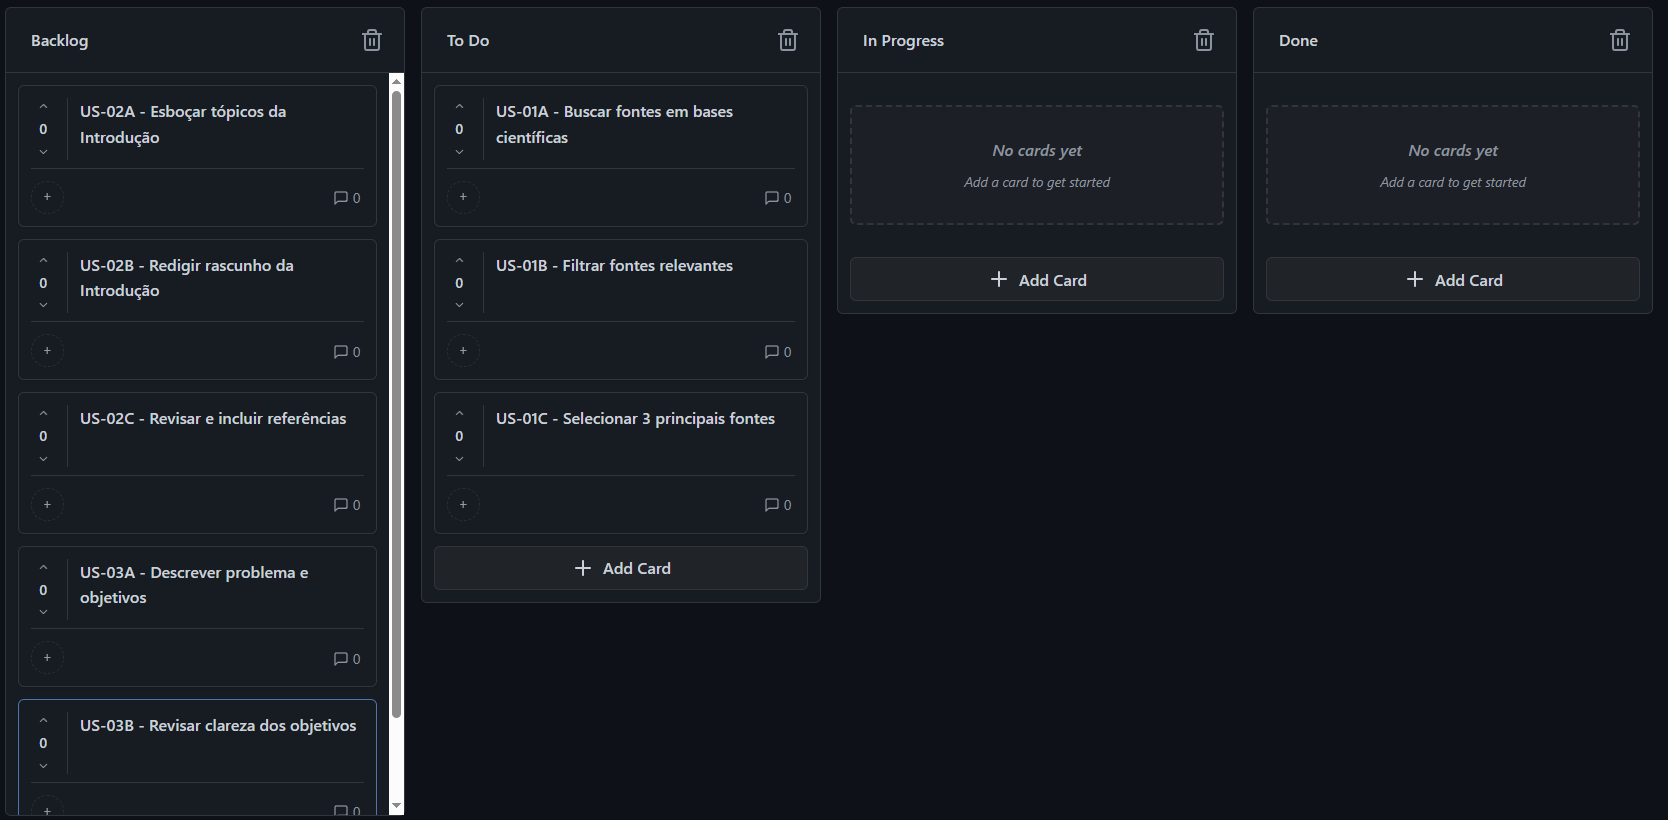
\includegraphics[width=0.8\linewidth]{pictures/kanban_sprint1_inicio.png}
  \caption{Visão geral do Quadro Kanban no início da Sprint 1}
\end{figure}

\begin{figure}[htbp]
  \centering
  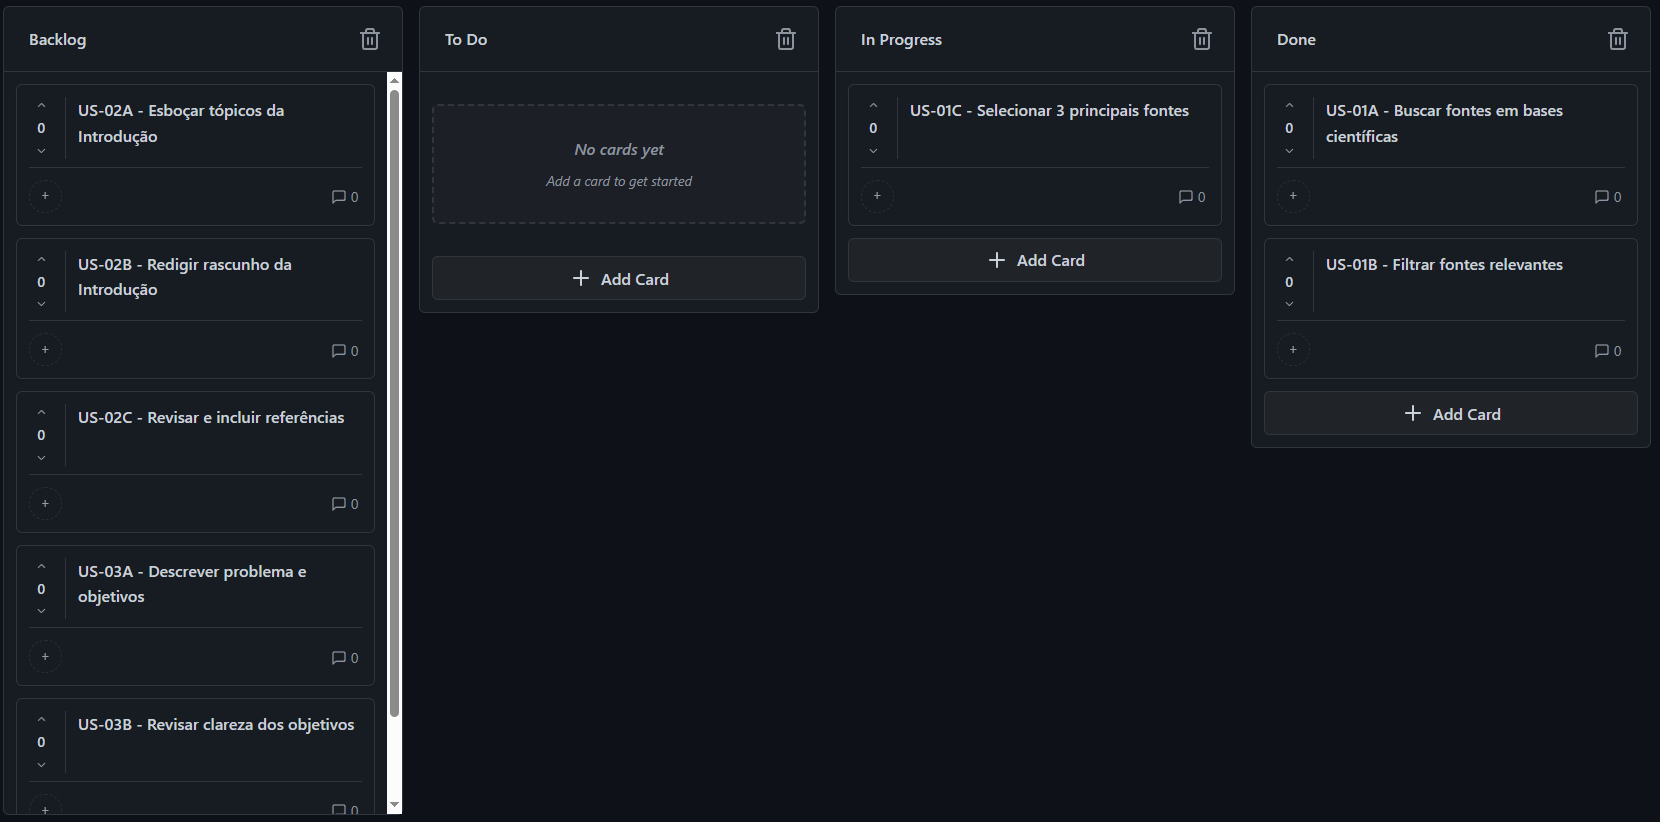
\includegraphics[width=0.8\linewidth]{pictures/kanban_sprint1_final.png}
  \caption{Visão geral do Quadro Kanban ao final da Sprint 1}
\end{figure}

\subsection{Reuniões de Acompanhamento}

Daily 1 (12/06/2025): Discutimos os critérios para filtragem de artigos e as ferramentas de busca mais eficazes.

Daily 2 (14/06/2025): Falta apenas a tarefa US-01C; Nota do futuro: a tarefa restante foi concluída em 17/06/2025, antes da retrospectiva.

\begin{figure}[htbp]
  \centering
  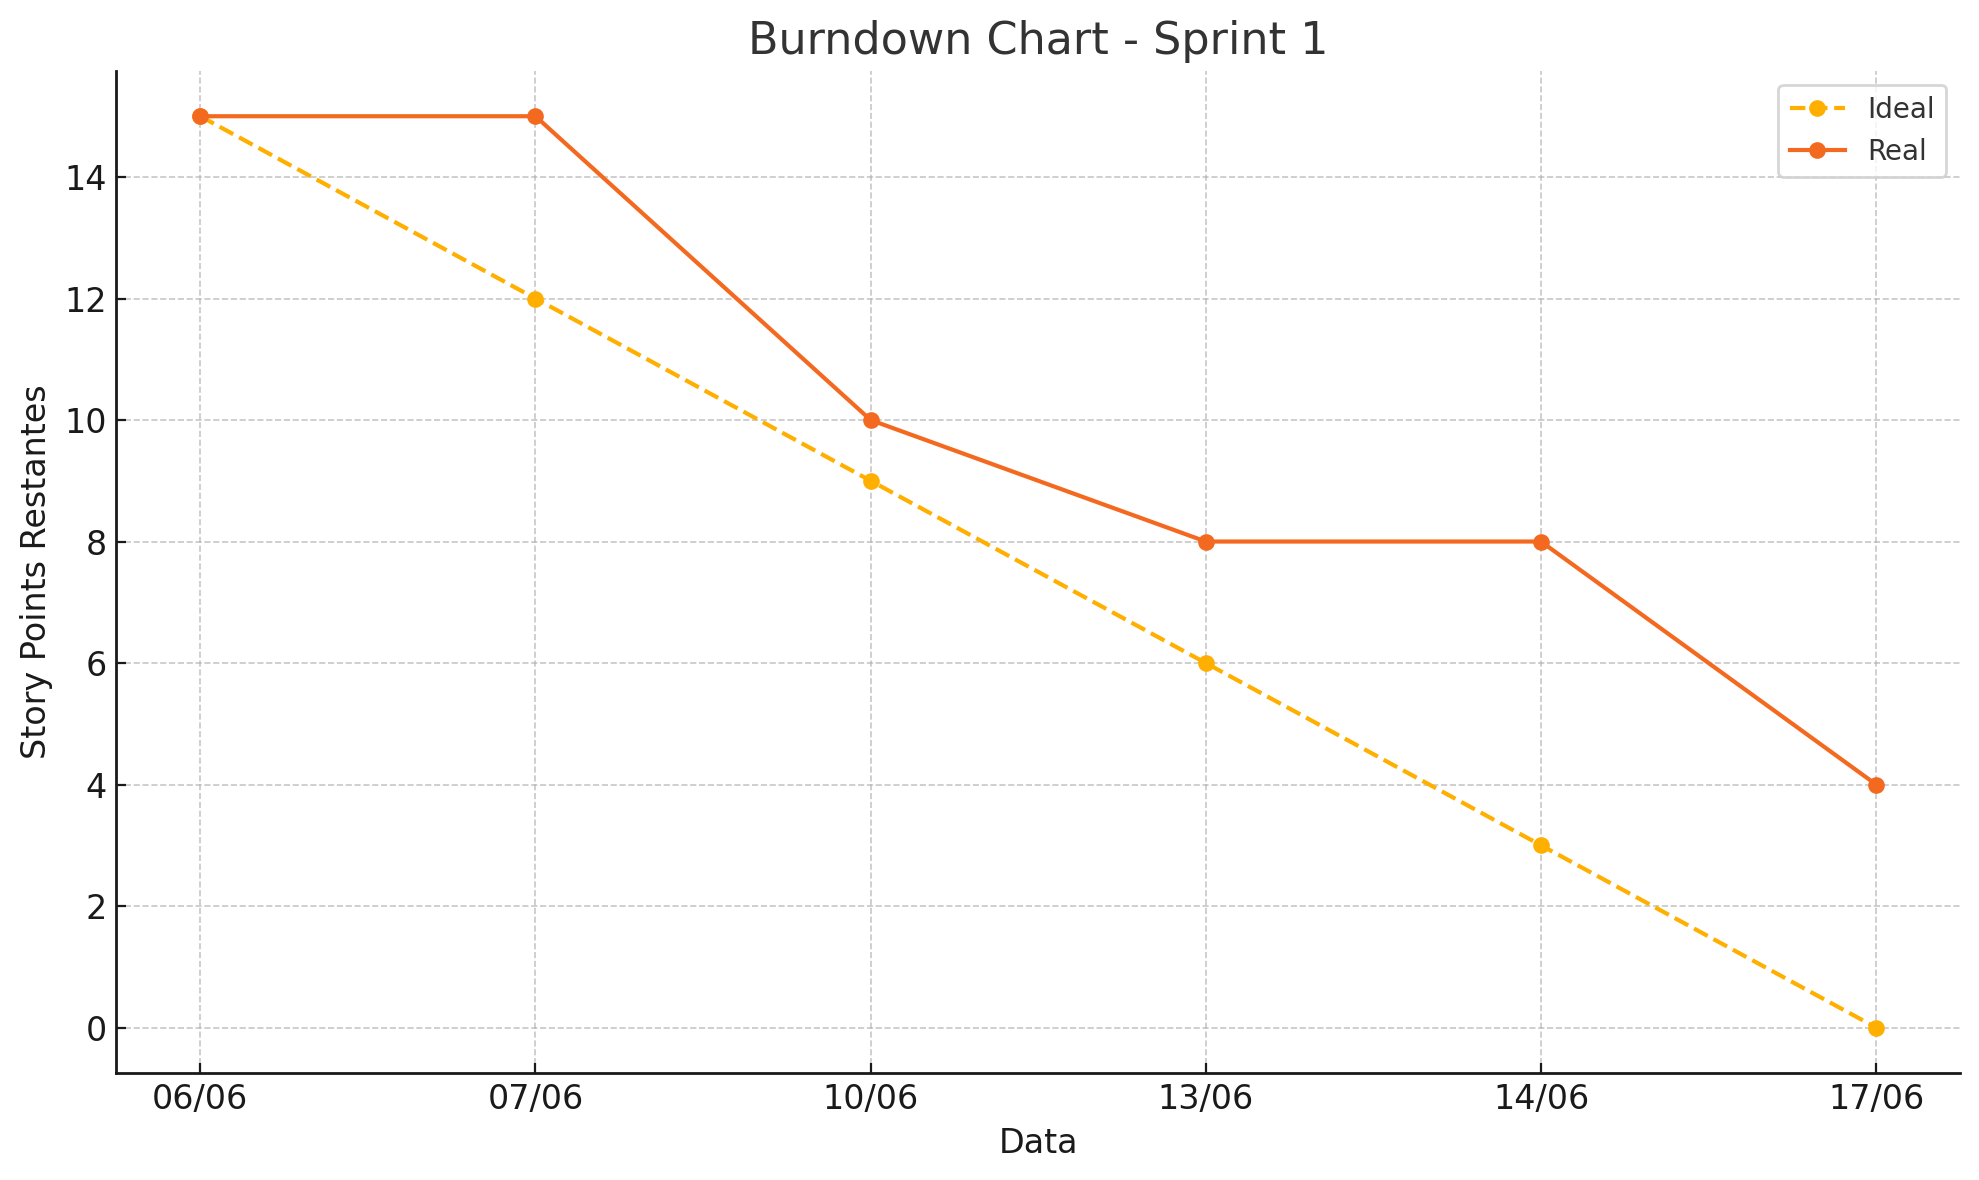
\includegraphics[width=0.7\linewidth]{pictures/burndown_sprint1.png}
  \caption{Burndown — Sprint 1}
\end{figure}


\subsection{Resultados das Sprints}

Essa teve como objetivo principal estruturar a base de fontes bibliográficas para o projeto. Todas as tarefas previstas foram concluídas, embora tenha havido desafios iniciais na definição de critérios de seleção. A equipe conseguiu identificar as três fontes principais a partir de um processo colaborativo de leitura e discussão.

\begin{table}[htbp]
  \centering
  \caption{Resultados — Sprint 1}
  \label{tab:resultSprint1}
  \begin{tabular}{lll}
    \toprule
    ID & Tarefas & Resultado \\
    \midrule
    US-01A & Buscar fontes & Concluída \\
    US-01B & Filtrar fontes & Concluída \\
    US-01C & Selecionar 3 principais fontes & Concluída em 17/06/2025 \\
    \bottomrule
  \end{tabular}
  \fonte{Elaboração própria.}
\end{table}

\vspace{1em}
\noindent\textbf{Resumo da Sprint:}
\begin{itemize}[noitemsep]
  \item Total de tarefas: 3
  \item Concluídas: 3
\end{itemize}

\subsection{Retrospectivas}

\begin{itemize}
  \item \textbf{Pontos de atenção}:
  \begin{itemize}
    \item Baixa adesão às reuniões intermediárias dificultou o alinhamento.
    \item Houve confusão inicial sobre critérios para selecionar artigos relevantes.
  \end{itemize}

  \item \textbf{O que pode ser melhorado}:
  \begin{itemize}
    \item Criar lembretes automáticos das reuniões.
    \item Alinhar expectativas sobre participação mínima esperada de cada integrante.
  \end{itemize}

  \item \textbf{O que manter/continuar}:
  \begin{itemize}
    \item Organização via checklist e Kanban funcionou bem.
    \item Leitura coletiva de fontes-chave ajudou a focar na qualidade da bibliografia.
  \end{itemize}
\end{itemize}

\vspace{1em}
\noindent\textbf{Burndown Chart:}

\begin{center}
  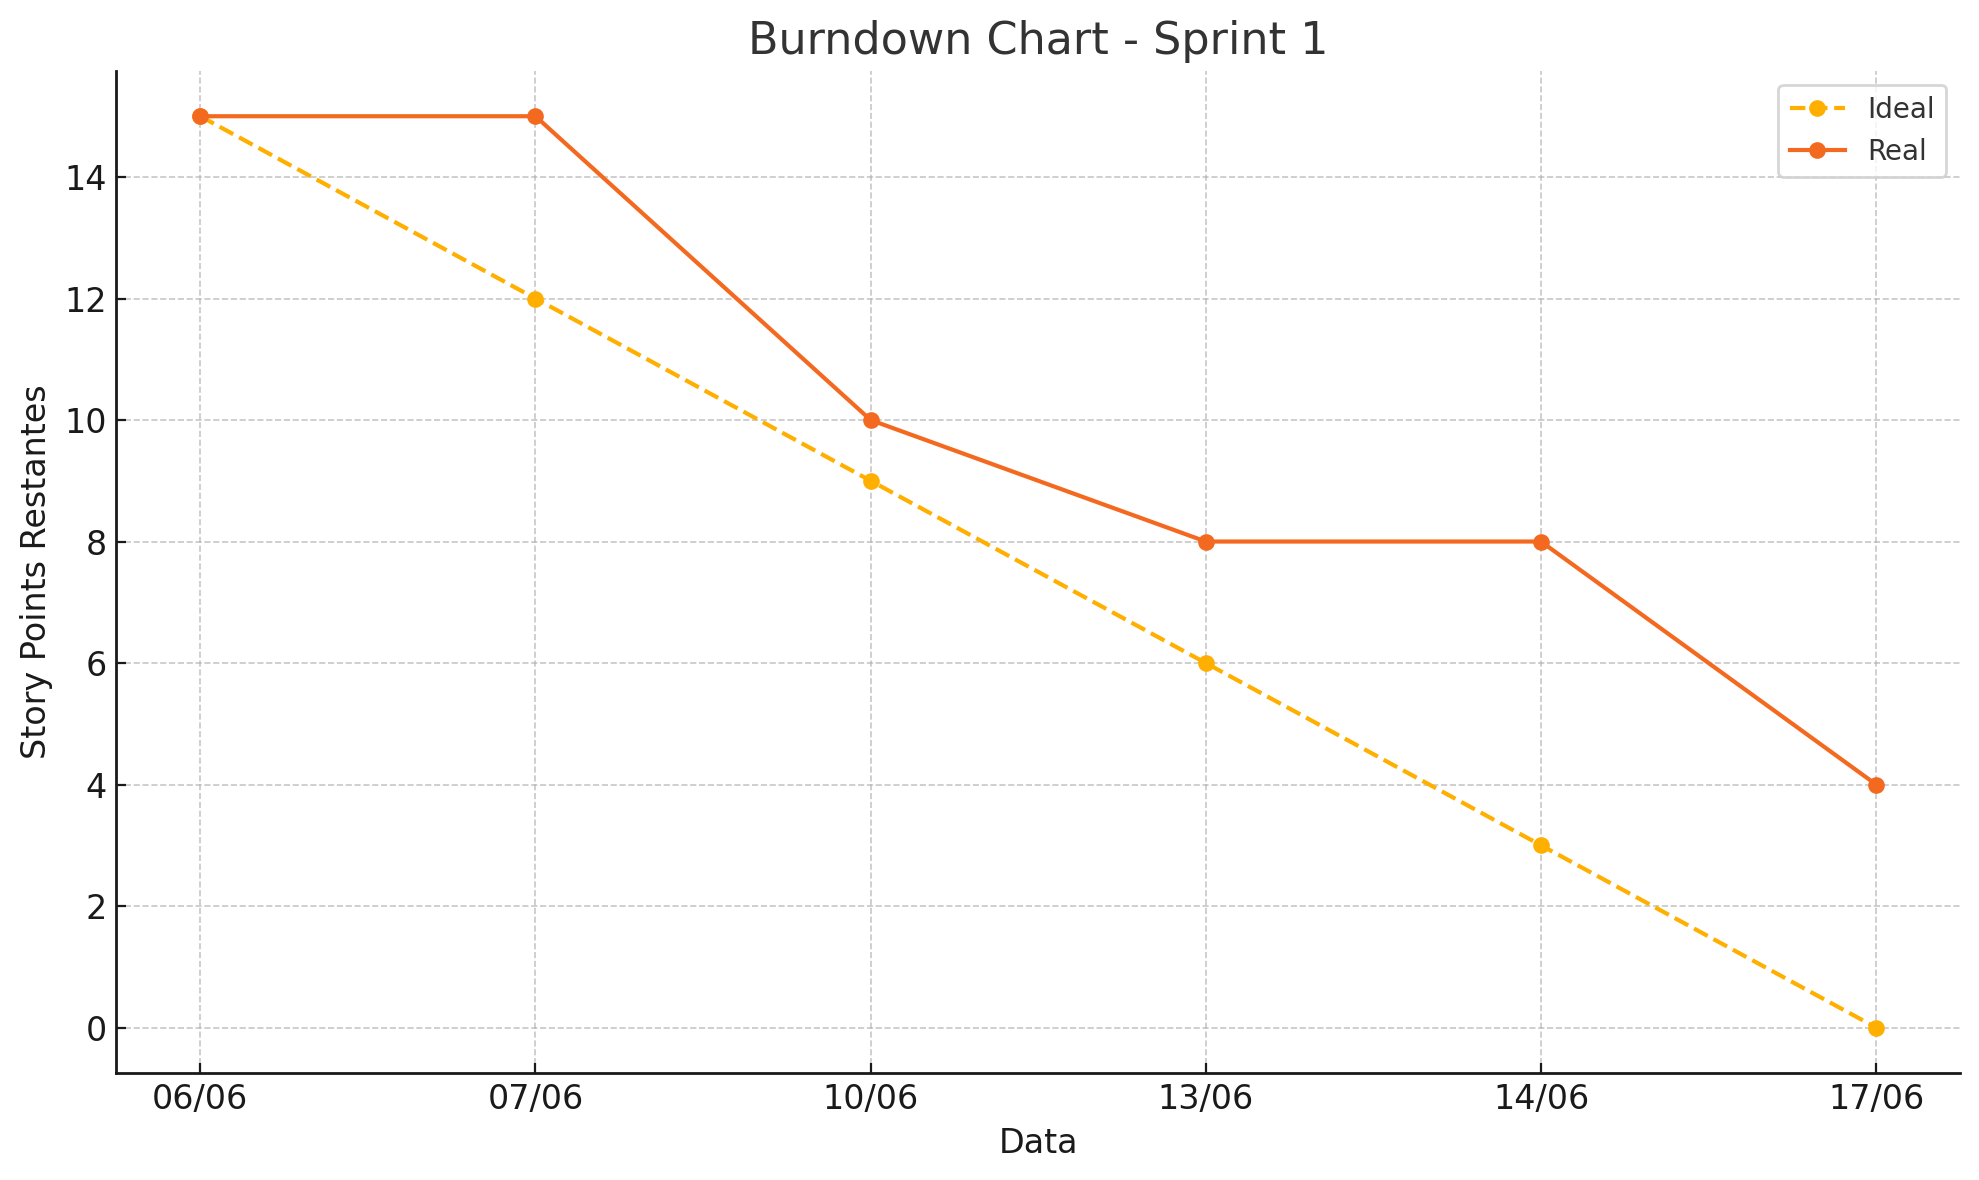
\includegraphics[width=0.8\textwidth]{pictures/burndown_sprint1.png}
\end{center}
\section{Sprint 2}

\subsection{Sprint Planning}

Objetivo da Sprint: Produzir a seção de Introdução da proposta de TCC e descrever claramente o problema e objetivos do trabalho.

\begin{table}[htbp]
  \centering
  \caption{Sprint backlog e tarefas — Sprint 2}
  \label{tab:sprint2}
  \begin{tabular}{ccc}
    \toprule
    Tarefa & Descrição & Estimativa (pessoas·hora) \\
    \midrule
    US-02A & Esboçar tópicos da Introdução & 2 \\
    US-02B & Redigir rascunho da Introdução & 4 \\
    US-02C & Revisar e incluir referências & 1 \\
    US-03A & Descrever problema e objetivos & 5 \\
    US-03B & Revisar clareza dos objetivos & 3 \\
    \bottomrule
  \end{tabular}
  \fonte{Elaboração própria.}
\end{table}

\vspace{0.5em}
\noindent\textbf{Capacidade utilizada:} 15 pessoas·hora (100\% da velocidade da equipe)

\subsection{Quadro Kanban}

Histórico da evolução do quadro Kanban no início e ao final de cada Sprint.

\begin{figure}[htbp]
  \centering
  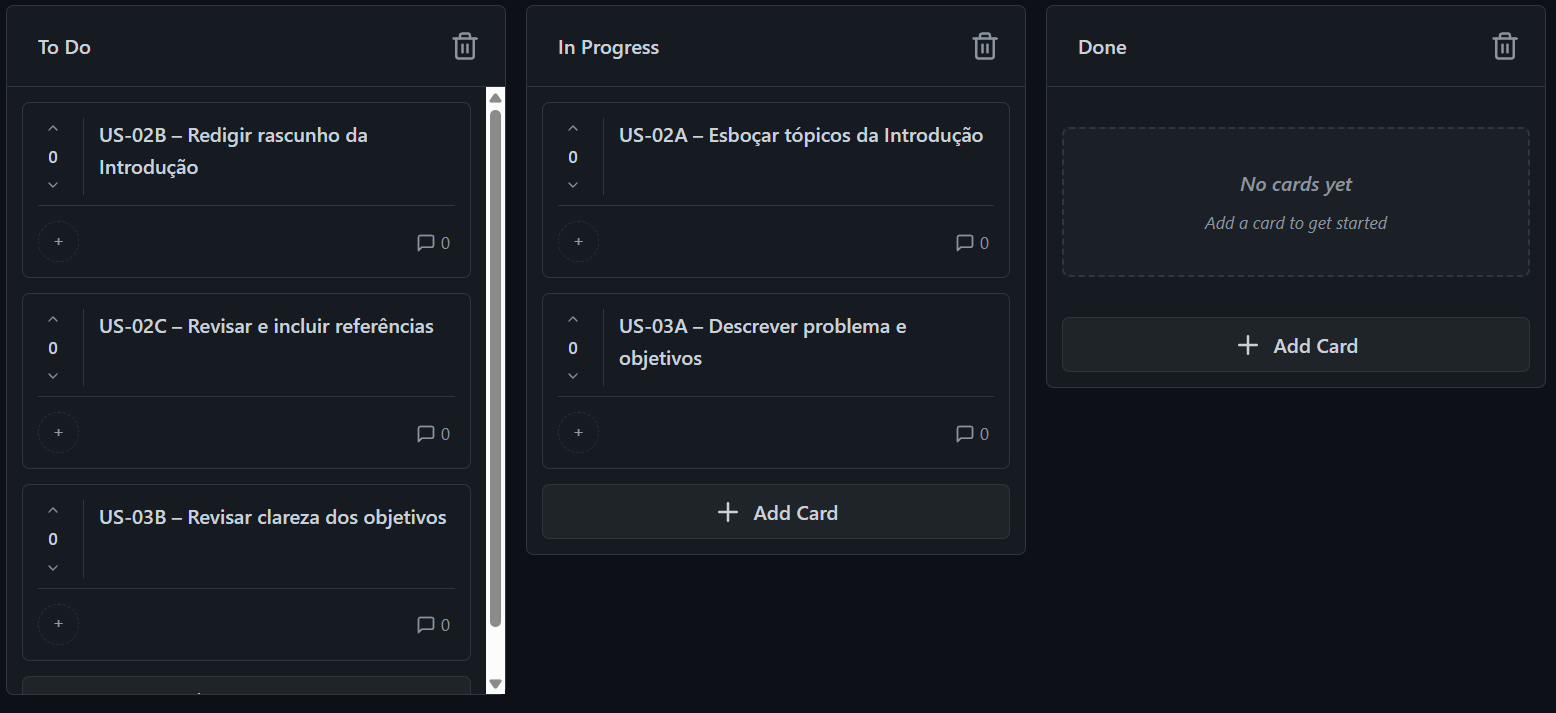
\includegraphics[width=0.8\linewidth]{pictures/kanban_sprint2_inicio.png}
  \caption{Visão geral do Quadro Kanban no início da Sprint 2}
\end{figure}

\begin{figure}[htbp]
  \centering
  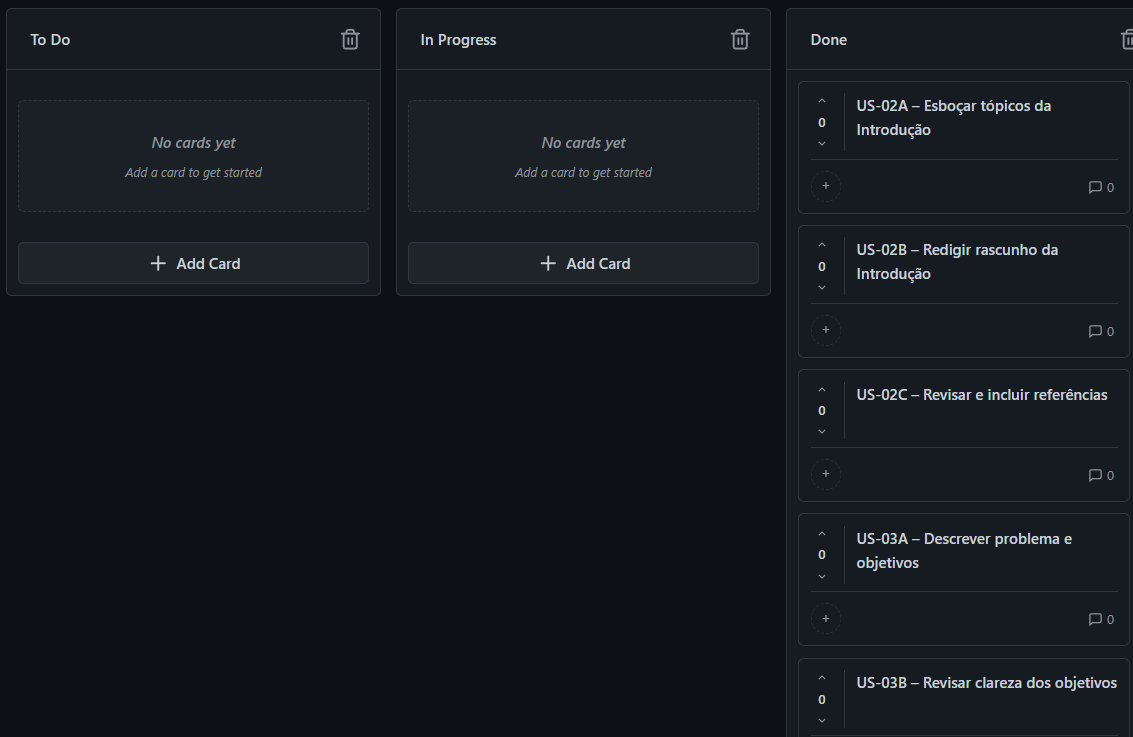
\includegraphics[width=0.8\linewidth]{pictures/kanban_sprint2_final.png}
  \caption{Visão geral do Quadro Kanban ao final da Sprint 2}
\end{figure}


\subsection{Reuniões de Acompanhamento}

Daily 3 (\textless Data\textgreater): Não houve.

\begin{figure}[htbp]
  \centering
  \includegraphics[width=0.6\linewidth]{pictures/daily3.png}
  \caption{Evidência da Daily 3}
\end{figure}

Daily 4 (21/06/2025): Todas as tarefas foram concluídas.

\begin{figure}[htbp]
  \centering
  
\includegraphics[width=0.6\linewidth]{pictures/daily4.png}
  \caption{Evidência da Daily 4}
\end{figure}

\begin{figure}[htbp]
  \centering
  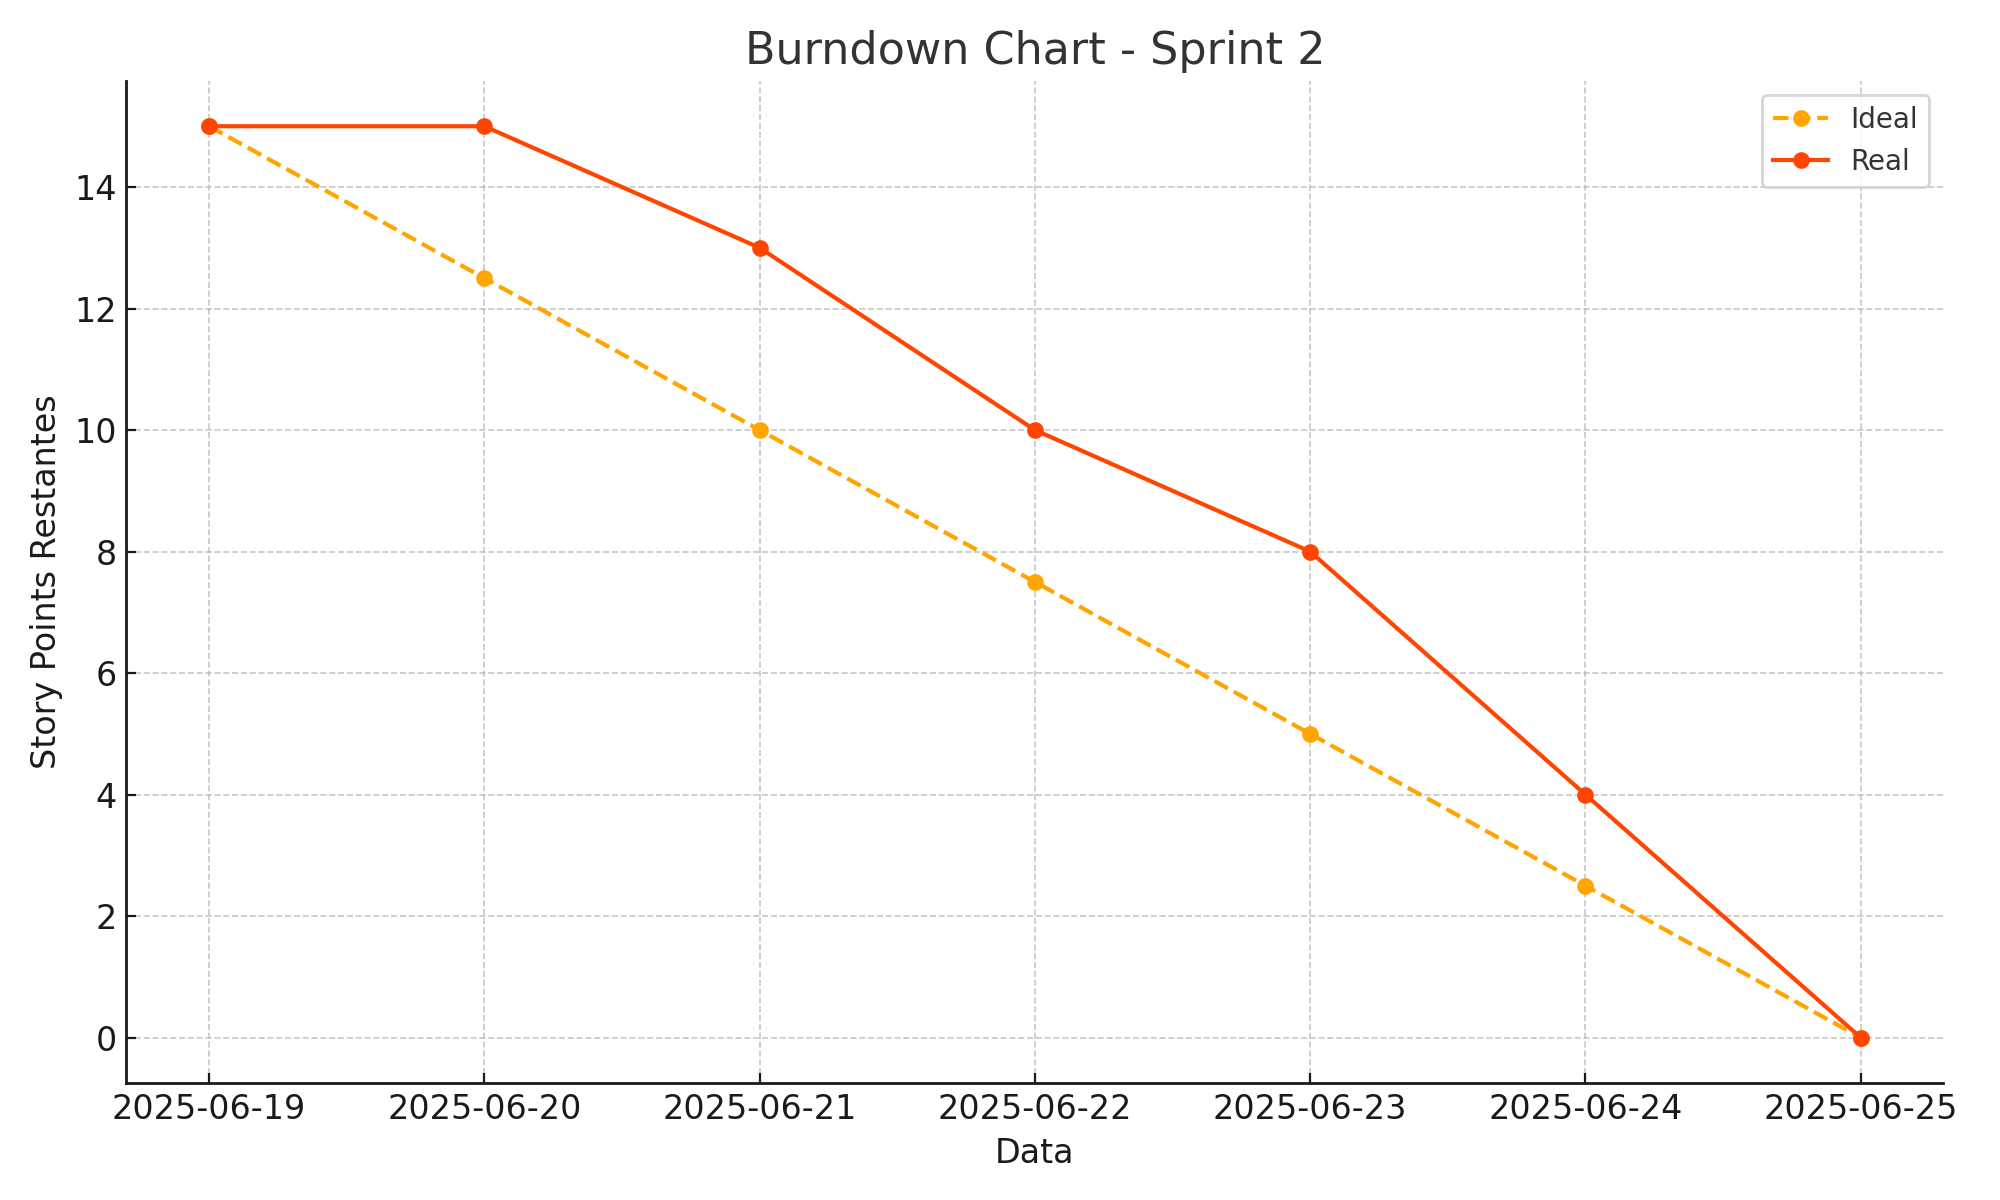
\includegraphics[width=0.7\linewidth]{pictures/burndown_sprint2.png}
  \caption{Burndown — Sprint 2}
\end{figure}



\subsection{Resultados das Sprints}

A Sprint 2 focou na redação da Introdução e na definição clara dos objetivos do trabalho. Apesar do escopo enxuto, a equipe conseguiu avançar de forma eficiente, finalizando a maior parte das tarefas planejadas. Identificou-se, no entanto, que seria possível assumir uma carga de trabalho maior.

\begin{table}[htbp]
  \centering
  \caption{Resultados — Sprint 2}
  \label{tab:resultSprint2}
  \begin{tabular}{lll}
    \toprule
    ID & Tarefa & Status \\
    \midrule
    US-02A & Esboçar tópicos da Introdução & Concluída \\
    US-02B & Redigir rascunho da Introdução & Concluída \\
    US-02C & Revisar e incluir referências & Concluída \\
    US-03A & Descrever problema e objetivos & Concluída \\
    US-03B & Revisar clareza dos objetivos & Concluída \\
    \bottomrule
  \end{tabular}
  \fonte{Elaboração própria.}
\end{table}

\vspace{1em}
\noindent\textbf{Resumo da Sprint:}
\begin{itemize}[noitemsep]
  \item Tarefas previstas: 5
  \item Concluídas: 5
\end{itemize}

\noindent\textbf{Aprendizados e observações:}
\begin{itemize}
  \item O escopo da sprint foi subestimado — poderia ter mais tasks.
\end{itemize}

% Evidências gráficas
\begin{figure}[htbp]
  \centering
  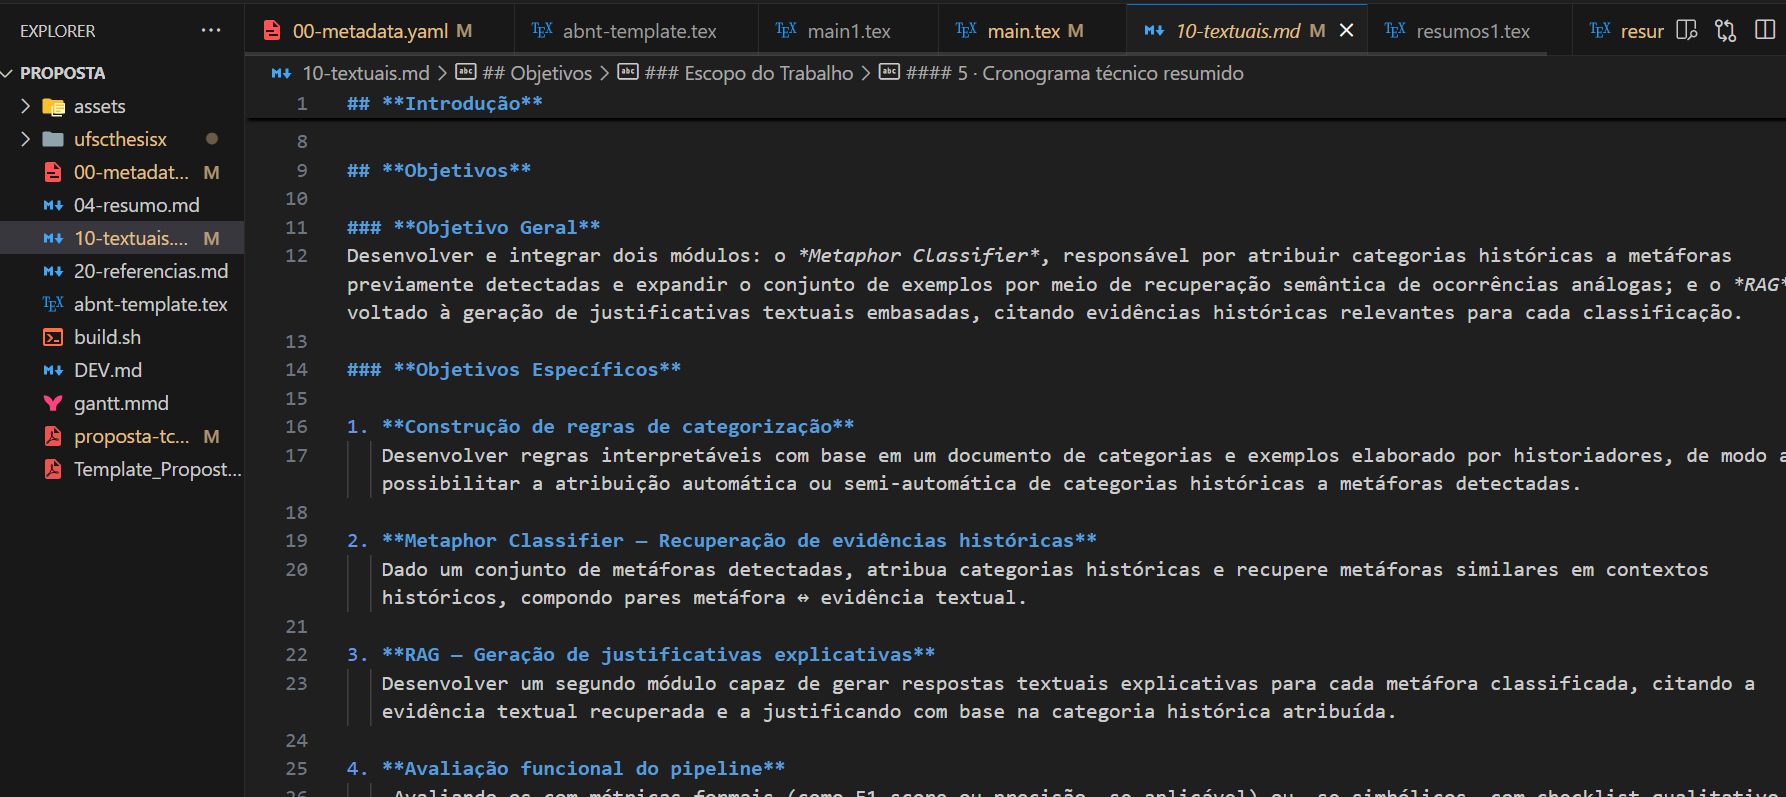
\includegraphics[width=0.6\linewidth]{pictures/intro_topicos.png}
  \caption{Evidência da tarefa US-02A}
\end{figure}

\begin{figure}[htbp]
  \centering
  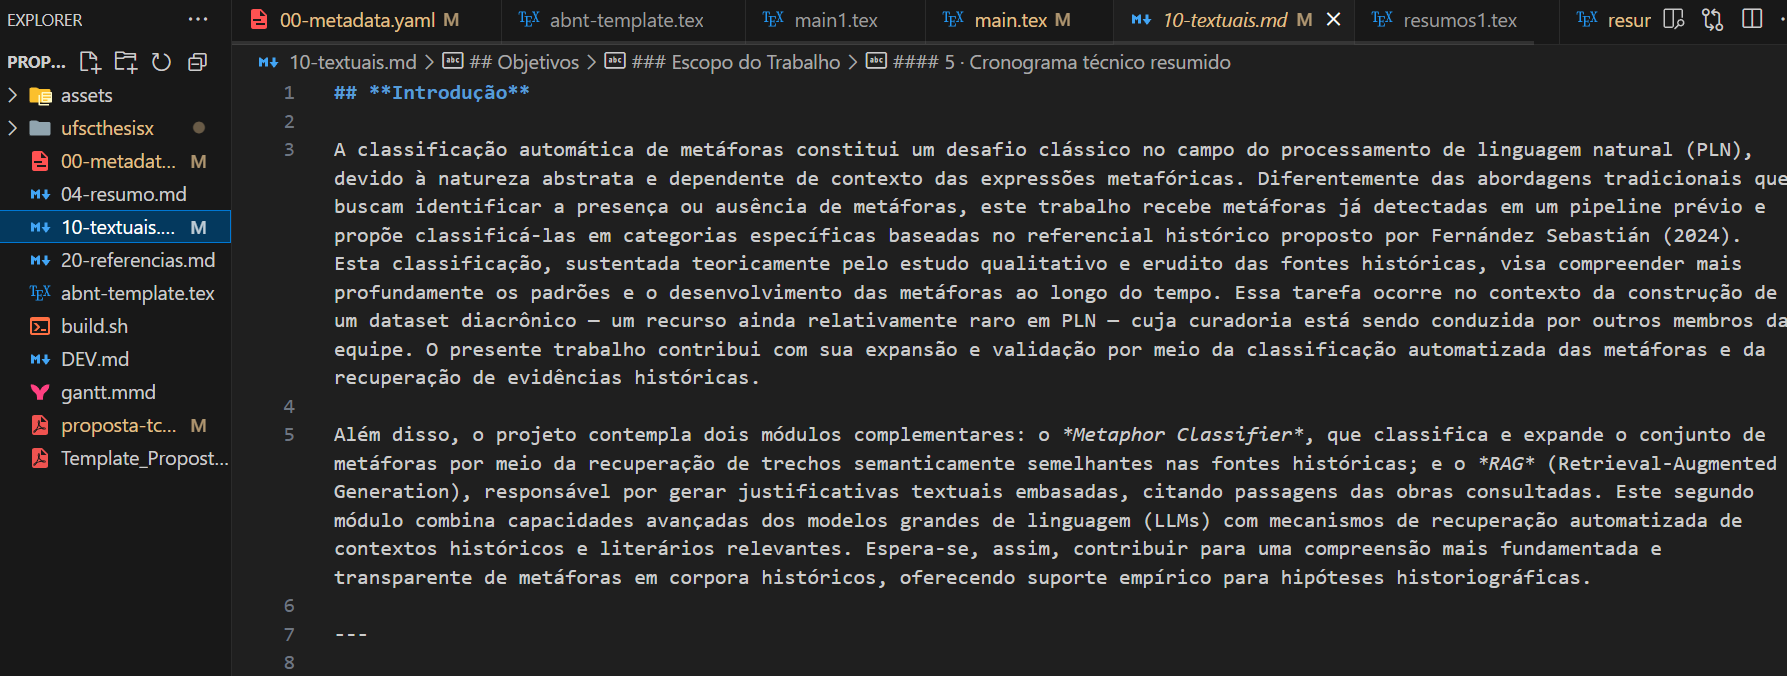
\includegraphics[width=0.6\linewidth]{pictures/intro_rascunho.png}
  \caption{Evidência da tarefa US-02B}
\end{figure}

\begin{figure}[htbp]
  \centering
  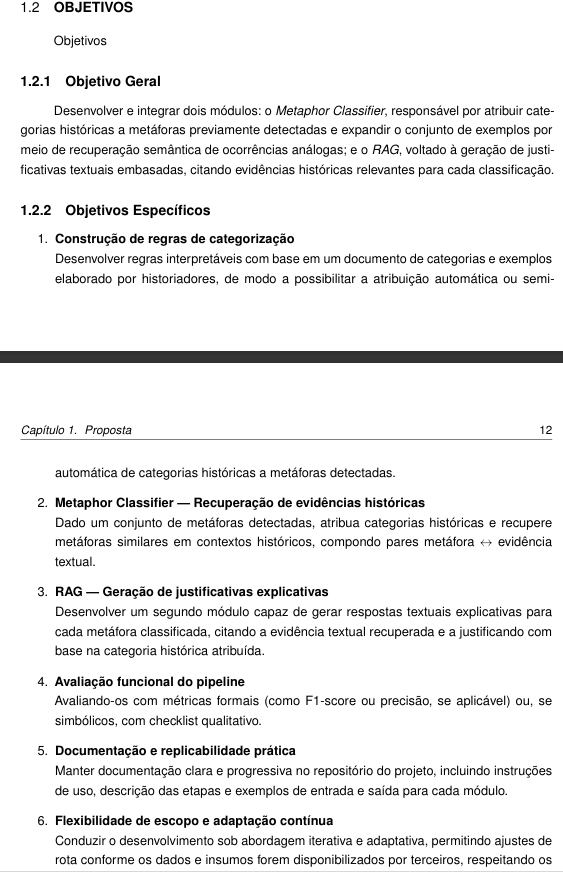
\includegraphics[width=0.6\linewidth]{pictures/problema_objetivos.png}
  \caption{Evidência da tarefa US-03A}
\end{figure}



\subsection{Retrospectivas}

\begin{itemize}
  \item \textbf{Pontos de atenção}:
  \begin{itemize}
    \item Houve apenas uma daily.
    \item O escopo da sprint foi subdimensionado: todas as tarefas foram concluídas rapidamente, sugerindo que seria possível incluir mais atividades.
  \end{itemize}

  \item \textbf{O que pode ser melhorado}:
  \begin{itemize}
    \item Garantir acompanhamento contínuo (respeitar as dailies).
    \item Refinar o planejamento de sprint com base na capacidade real do grupo, prevendo mais tarefas quando possível.
  \end{itemize}

  \item \textbf{O que manter/continuar}:
  \begin{itemize}
    \item Boa execução e comprometimento da equipe com as entregas.
    \item Clareza nos objetivos da sprint facilitou o foco e a conclusão eficiente das tarefas.
  \end{itemize}
\end{itemize}

\vspace{1em}
\noindent\textbf{Burndown Chart:}

\begin{center}
  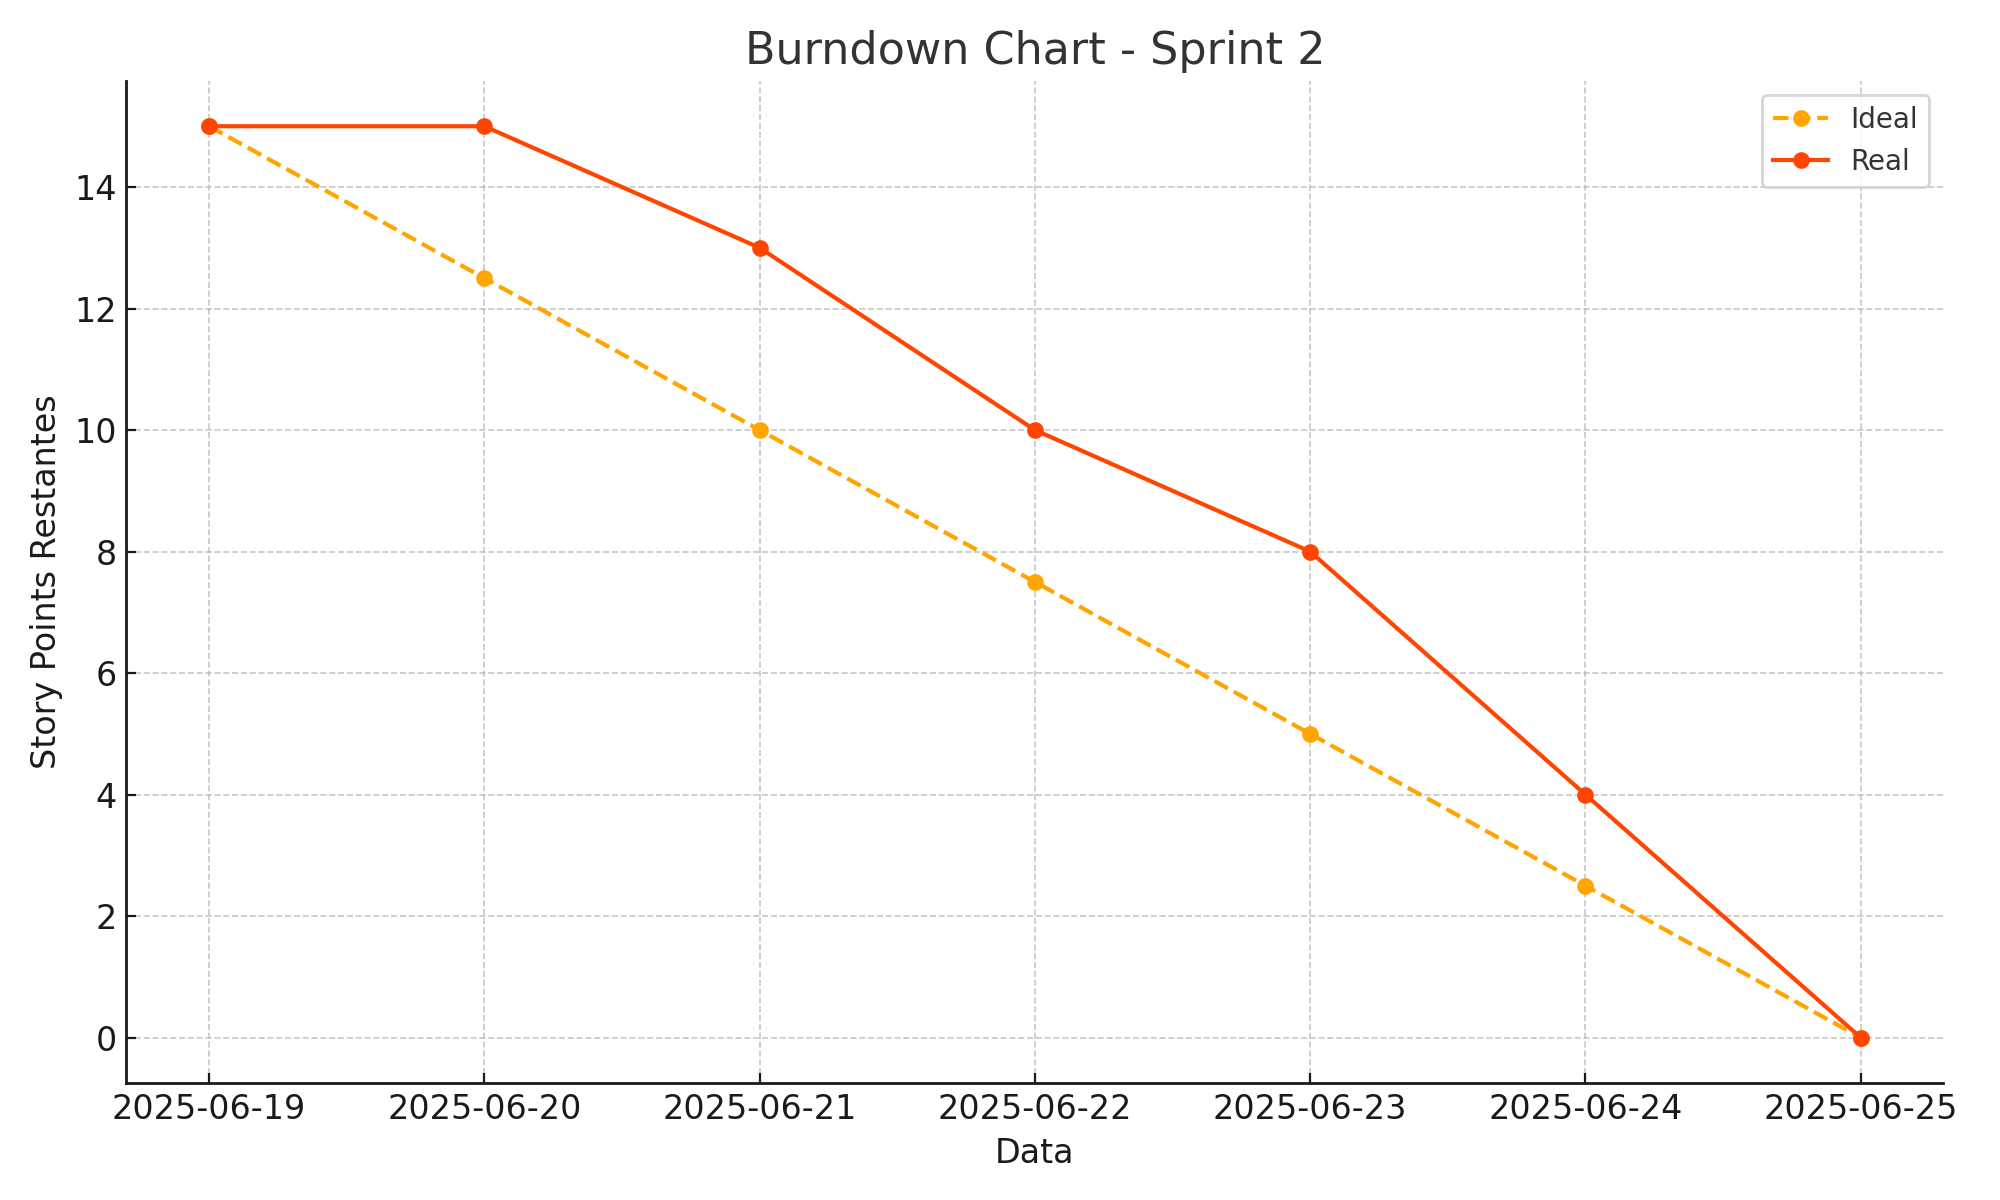
\includegraphics[width=0.8\textwidth]{pictures/burndown_sprint2.png}
\end{center}


\end{document}
